\chapter{Materiais e Métodos}
	\label{materiaisEMetodos}

	Para a concretização deste trabalho, são necessários materiais tanto de ordem computacional, para processamento e implementação de software, tanto de ordem de dados, principalmente para teste das hipóteses encontradas, verificação de sucesso e embasamento teórico. 
	
	Os materiais em forma de dados devem consistir, basicamente, em imagens de objetos isolados e, de preferência, com elementos dispensáveis como plano de fundo e texturas padronizados e sistema ortogonal de coordenadas de referência, a fim de facilitar o processamento dos dados pelo computador e o funcionamento dos algoritmos desenvolvidos; foi conseguido um número suficiente, para o início do trabalho, de imagens que correspondiam a este padrão desejado através de repositórios \textit{on-line}. 
	
	A demanda por recursos computacionais de alta eficiência é baixa, portanto, pode-se, utilizar o computador pessoal do autor sem prejuízo de tempo; além disto, serão utlizadas ferramentas computacionais de terceiros, como bibliotecas de linguagens de programação e ambientes de edição de código-fonte, sob licença acadêmica gratuita, portanto, não acarretando em custos financeiros para a execução do trabalho.
	
	Tendo em vista o escopo bem definido e a um conjunto de materiais de aplicação estrito deste trabalho, foi buscado um método de desenvolvimento adequado à esta produção que, por não visar a solução de um problema de grande amplitude no universo da computação gráfica, pode ser dito como enxuto. A escolha considerada apropriada para tal cenário de trabalho é a metodologia Lean, também chamada de metodologia Enxuta.
	
\section{Recursos Computacionais}

	Não havendo grande volume de dados ou alta complexidade no processamento dos dados, será utilizado o computador pessoal textit{Notebook} Mobile Sim+ 6220 do autor do trabalho, com a seguinte configuração:
\begin{itemize}
	\item processador Intel\textregistered Core\textregistered i3 330M (2,13 GHz, 3MB Cache);
	\item memória RAM Kingston\textregistered PC3-8500 (4MB, DDR3);
	\item chipset gráfico Intel\textregistered HM55;
	\item sistema operacional Windows 7\textregistered.
\end{itemize}

	Para fins de construção de programas de computador e otimização do rendimento dos códigos-fontes em relação ao \textit{hardware} disponível, serão usadas as seguintes ferramentas computacionais:
\begin{itemize}
	\item Ambiente gráfico para programação em linguagem C\# Microsoft Visual Studio 2010 v4.5.50938 RTMRel\textregistered;
	\item Biblioteca de métodos algébricos em C\# ALGLIB Free Edition v3.8.2
	\item Software de visualização 3D Meshlab v1.3.3.
\end{itemize}

\section{Conjunto de Dados}
	\label{secaoConjuntoDeDados}

	Os dados utilizados como entrada nos algoritmos e programas desenvolvidos neste trabalho consistem em imagens digitais representando objetos apresentados no capítulo \ref{introducao}, o \textit{VW Beetle} de Sutherland (figura \ref{sutherlandVWDuplo}), o Bule de Leite de Newell (figura \ref{utahMilkjugDuplo}) e uma litografia digitalizada de Dürer (figura \ref{durerPerspectiva}). Todas as imagens utilizadas neste trabalho foram obtidas respeitando os direitos autorais e de reprodução.
	
	Quanto ao \textit{VW Beetle} de Sutherland, conseguiu-se obter uma imagem com sistemas ortogonais de coordenadas de referência graficamente evidentes (figura \ref{sutherlandVWDuplo3}), no entanto todas as imagens apresentavam-se em projeção em perspectiva, distorcendo as linhas do sistema de referência. Todas as imagens referentes a este objeto apresentavam regiões desprezíveis, como plano de fundo, facilmente diferenciáveis através de cor. Em formato `JPG', as imagens possuíam resolução de 72 dpi e 24 bits para intensidade de cor.

\begin{figure}[!htb]
	\centering
	\subfloat[\textit{VW Beetle} de Sutherland renderizado \cite{renderingSutherlandVW}]{
		\includegraphics[height=5cm]{imagens/SutherlandsVW-Skinned.jpg}
		\label{sutherlandVWDuplo1}
	}
	\quad
	\subfloat[\textit{VW Beetle} de Sutherland em \textit{wireframe} \cite{wireframeSutherlandVW}]{
		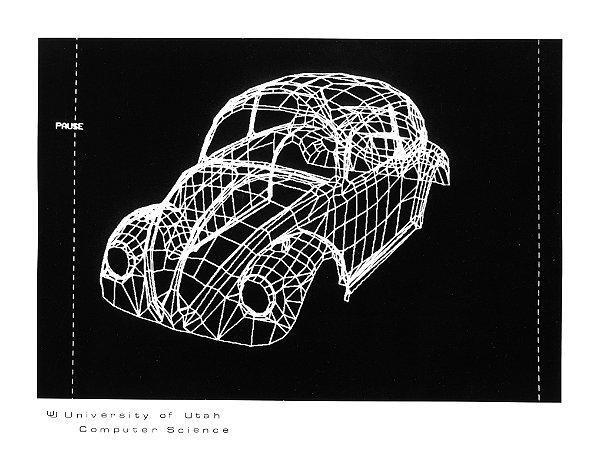
\includegraphics[height=5cm]{imagens/SutherlandsVW-Wireframe.jpg}
		\label{sutherlandVWDuplo2}
	}
	\quad
	\subfloat[\textit{VW Beetle} de Sutherland com referências \cite{jalopnik}]{
		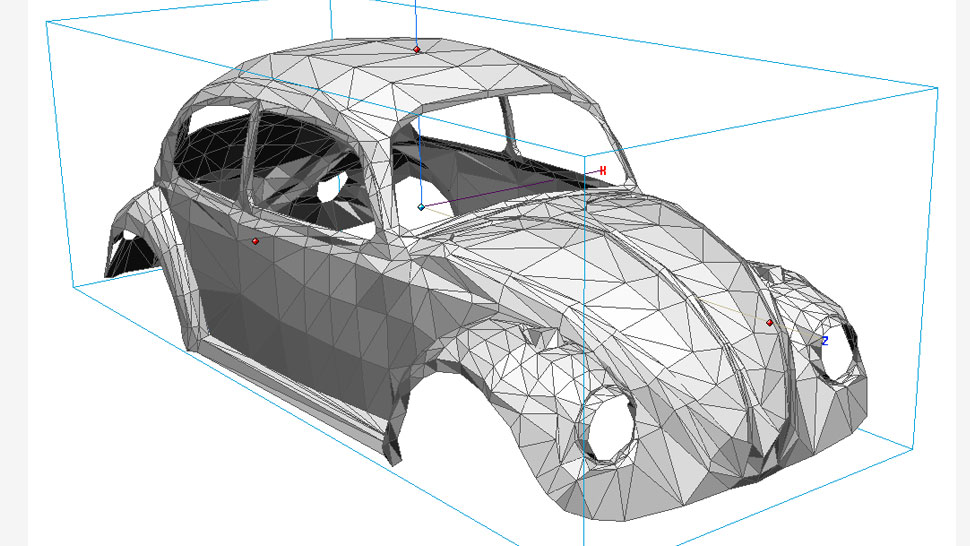
\includegraphics[height=5cm]{imagens/SutherlandsVW-Skinned-Referenced.jpg}
		\label{sutherlandVWDuplo3}
	}
	\caption{O \textit{VW Beetle} de Sutherland}
	\label{sutherlandVWDuplo}
\end{figure}
	
	As imagens do Bule de Leite de Newell, por este ser um objeto sem registro oficial dos seus dados, são menos elaboradas, com o sistema de coordenadas de referência mais nebuloso, mas, afortunadamente, apresentando projeção paralela isométrica. Tais imagens são em branco e preto, em formato `PNG' com 32 bits para intensidade de cor e resolução de 95 dpi.

\begin{figure}[!htb]
	\centering
	\subfloat[Bule de Leite de Newell convencional \cite{newellResearch}]{
		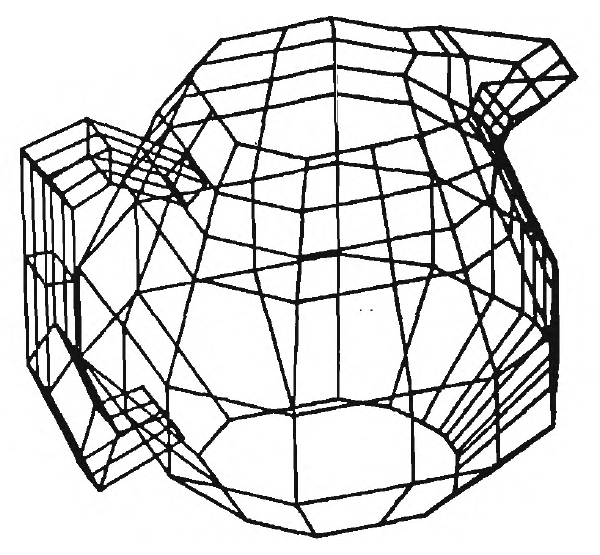
\includegraphics[height=5cm]{imagens/Milkjug-Wireframe-1.png}
		\label{utahMilkjugDuplo1}
	}
	\quad
	\subfloat[Bule de Leite de Newell suavizado \cite{newellResearch}]{
		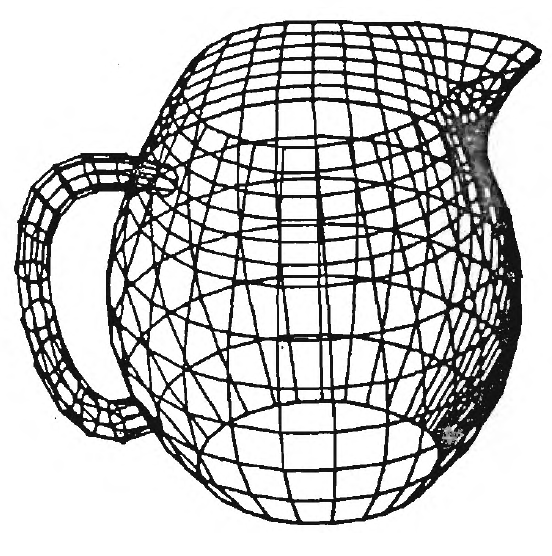
\includegraphics[height=5cm]{imagens/Milkjug-Wireframe-2.png}
		\label{utahMilkjugDuplo2}
	}
	\caption{O Bule de Leite de Newell}
	\label{utahMilkjugDuplo}
\end{figure}

	A litografia de Dürer, digitalizada e disponibilizada por terceiros, possui um sistema de referências evidente e, como se pode prever, está representada através da projeção em perspectiva. Em formato `JPG' com 96 dpi de resolução e 24 bits de profundidade de cor.
	
\begin{figure}[!htb]
	\centering
	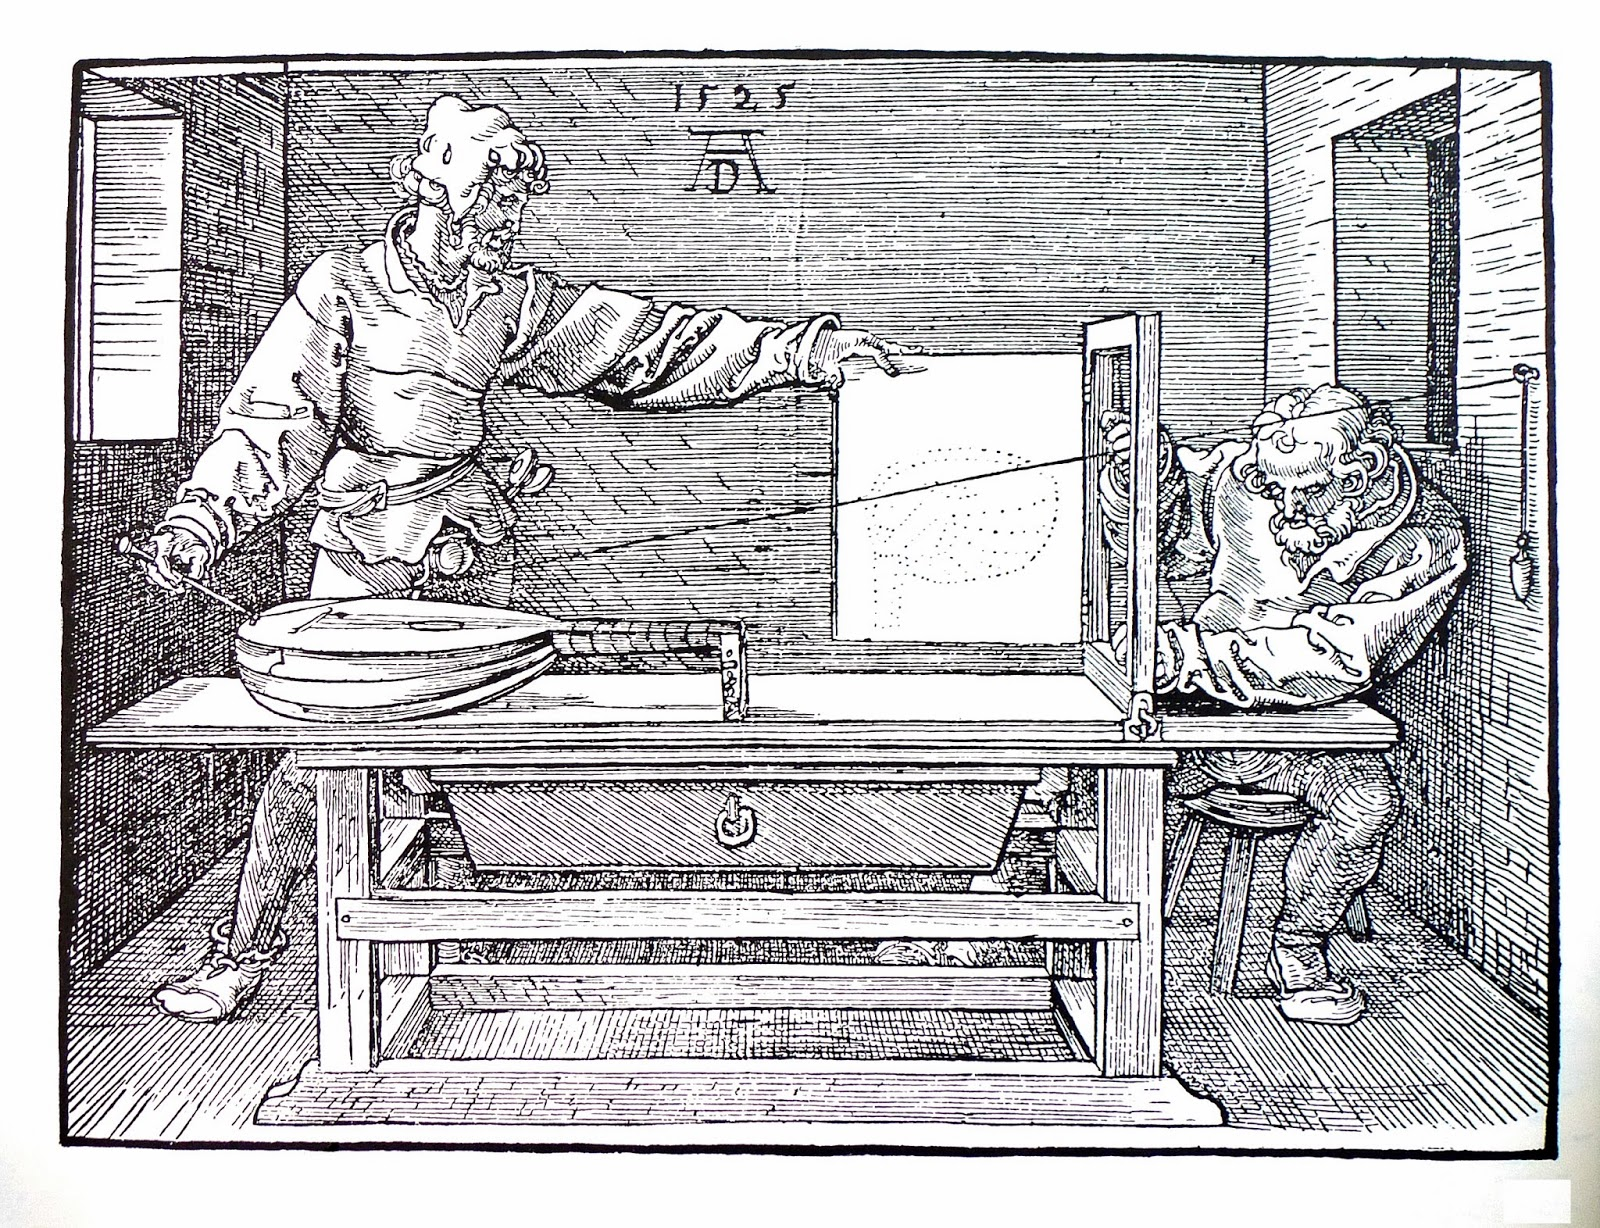
\includegraphics[height=7cm]{imagens/durer.jpg}
	\caption{A litografia de Dürer \cite{durerSite}}
	\label{durerPerspectiva}
\end{figure}
	
\section{Aferição da corretude}

	Como o objetivo deste trabalho é reconstruir objetos cujas informações tridimensionais são inexistentes, é impossível se fazer uma validação direta dos resultados obtidos, isto é, não há como comparar os modelos tridimensionais obtidos neste trabalho com um modelo paramétrico dos mesmos objetos estudados.

	De tal forma, a corretude dos modelos obtidos será obtida de forma implícita, através da validação da técnica de reconstrução deste trabalho. Utilizando cenas específicas confeccionadas pelo autor (figuras \ref{cenasValidacao}), nas quais os elementos a serem reconstruídos têm suas informações catalogadas, será estimado um erro geométrico $E$ (fórmula \ref{formulaErroGeometricoMedio}) entre os pontos de coordenadas conhecidos dos modelos (P) e os pontos de coordenadas obtidos pela técnica desenvolvida neste trabalho (P'). 
	
\begin{equation}
	\label{formulaErroGeometricoMedio}
	E = \sqrt{(x_{P_i} - x_{P'_i})^2 + (y_{P_i} - y_{P'_i})^2 + (z_{P_i} - z_{P'_i})^2} 
\end{equation}
	
\begin{figure}[!htb]
	\centering
	\subfloat[Cena específica 1, um cubo unitário]{
		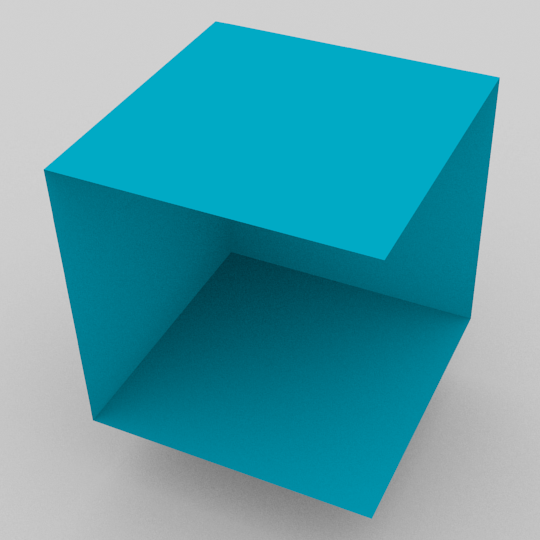
\includegraphics[height=4cm]{imagens/cenaTeste1.png}
		\label{cenaValidacao1}
	}
	\quad
	\subfloat[Cena específica 2, uma pirâmide regular equilátera unitária]{
		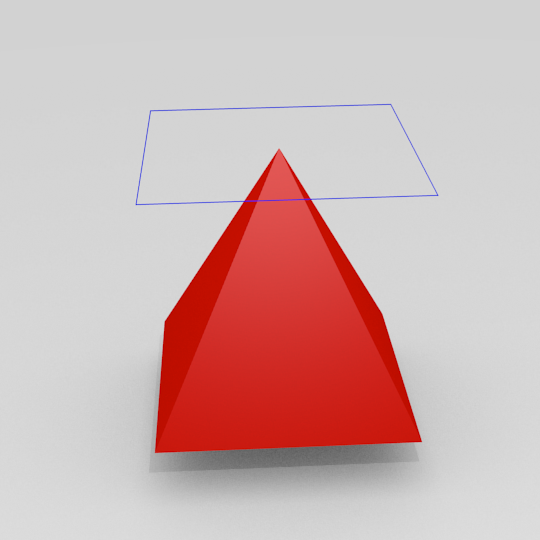
\includegraphics[height=4cm]{imagens/cenaTeste2.png}
		\label{cenaValidacao2}
	}
	\quad
	\subfloat[Cena específica 3, um cubo de dimensão $0.5$]{
		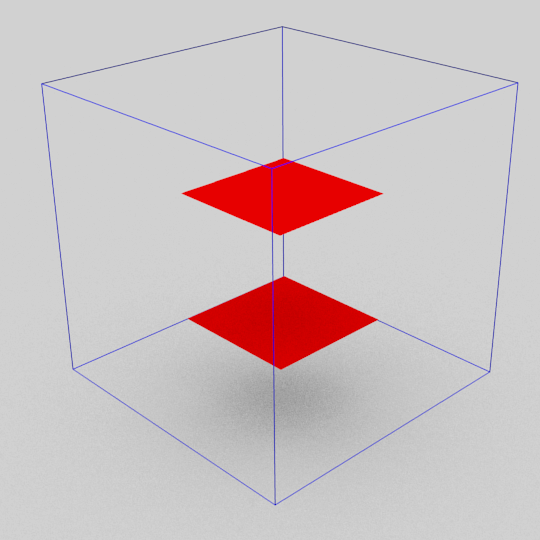
\includegraphics[height=4cm]{imagens/cenaTeste3.png}
		\label{cenaValidacao3}
	}
	\caption{Cenas para validação da técnica de reconstrução}
	\label{cenasValidacao}
\end{figure}

	Com a cena de validação 1 (figura \ref{cenaValidacao1}) deseja-se a reconstrução dos vértices de um hexaedro de dimensão unitária; com a cena de validação 2 (figura \ref{cenaValidacao2}) almejam-se os vértices de uma pirâmide regular equilátera de dimensão unitária; por fim, com a cena de validação 3, buscam-se os vértices de um cubo de dimensão $0.5$. 
	
	Nas cenas de validação há um plano abaixo do objeto descrito anteriormente, este não será reconstruído, servindo apenas como aparato visual na imagem da cena. Na cena de validação 1 (figura \ref{cenaValidacao1}), um cubo (hexaedro) teve duas de suas faces removidas, a fim facilitar a demarcação de pontos de referência, originando a figura vista. No caso da figura \ref{cenaValidacao2}, há, ainda, um quadrado de cor azul paralelo ao plano da base da pirâmide; tal quadrado é um auxílio, inserido pelo autor, para a demarcação dos pontos de referência e também será desconsiderado como objeto em reconstrução. A figura \ref{cenaValidacao3}, por sua vez, apresenta as arestas (em azul) de um cubo, estas são um auxílio para a demarcação de referências; note que neste cena também foram removidas faces do cubo para facilitar demarcações.

	Todas as imagens das cenas de validação têm resolução de 72 dpi.